\title{Aula 13 - TLS}

\author{Prof. Gabriel Rodrigues Caldas de Aquino}

\institute
{
    Instituto de Computação \\
    Universidade Federal do Rio de Janeiro\\
    gabrielaquino@ic.ufrj.br% Your institution for the title page
}
\date{Compilado em: \\ \today} % Date, can be changed to a custom date

%----------------------------------------------------------------------------------------
%    PRESENTATION SLIDE
%----------------------------------------------------------------------------------------



\begin{frame}
    % Print the title page as the first slide
    \titlepage
\end{frame}

\begin{frame}{Protegendo conexões TCP: TLS}
    \begin{itemize}
        \item \textbf{Contextualização:}
              \begin{itemize}
                  \item Vimos segurança na camada de rede.
                  \item Agora, subimos uma camada na pilha de protocolo.
              \end{itemize}

        \item \textbf{O Objetivo do TLS:}
              \begin{itemize}
                  \item Examinar como a criptografia pode aprimorar o \textbf{TCP}.
                  \item (Transport Layer Security).
              \end{itemize}

        \item \textbf{Serviços de Segurança Adicionados ao TCP:}
              \begin{itemize}
                  \item Sigilo (Confidencialidade).
                  \item Integridade dos Dados.
                  \item Autenticação do Ponto Final (End-point Authentication).
              \end{itemize}

        \item \textbf{Padronização e Histórico:}
              \begin{itemize}
                  \item O TLS é padronizado pelo IETF na \textbf{RFC 4346}.
                  \item Uma versão anterior e semelhante deste protocolo é o \textbf{SSL (Secure Sockets Layer)} versão 3.
              \end{itemize}
    \end{itemize}
\end{frame}

\begin{frame}{TLS: Histórico e Adoção}
    \begin{itemize}
        \item \textbf{Origem:} O SSL (Secure Sockets Layer) foi originalmente projetado pela Netscape.
              \begin{itemize}
                  \item (Ideias básicas sobre proteção do TCP antecedem este trabalho, ex: Woo, 1994).
              \end{itemize}

        \item \textbf{Sucessor:} O TLS (Transport Layer Security) é o sucessor padronizado do SSL.

        \item \textbf{Adoção Massiva:}
              \begin{itemize}
                  \item Suportado por todos os navegadores Web e servidores Web populares.
                  \item Usado pelo Gmail e por \textbf{basicamente todos os sites de comércio eletrônico} (Amazon, eBay, TaoBao).
                  \item Centenas de bilhões de dólares são gastos anualmente usando TLS.
              \end{itemize}

        \item \textbf{Como o usuário identifica o TLS?}
              \begin{itemize}
                  \item Se você já comprou algo online com cartão de crédito, sua comunicação foi quase certamente via TLS.
                  \item A URL no navegador se inicia com \textbf{https://} (em vez de http://).
              \end{itemize}
    \end{itemize}
\end{frame}

\begin{frame}{A Necessidade do TLS: Cenário de E-commerce}
    \begin{itemize}
        \item \textbf{O Cenário Típico:}
              \begin{itemize}
                  \item \textbf{Bob} (cliente) está navegando na Web.
                  \item Ele acessa o site da \textbf{Alice Incorporated} (vendedor) para comprar perfume.
              \end{itemize}

        \item \textbf{A Ação:}
              \begin{itemize}
                  \item O site exibe um formulário.
                  \item Bob insere informações sensíveis:
                        \begin{itemize}
                            \item Tipo de perfume e quantidade.
                            \item Seu endereço.
                            \item O \textbf{número de seu cartão de crédito}.
                        \end{itemize}
                  \item Bob clica em "Enviar".
              \end{itemize}

        \item \textbf{A Expectativa (sem segurança):}
              \begin{itemize}
                  \item Bob espera receber o perfume e a cobrança correta.
                  \item \textbf{O Risco:} Se nenhuma medida de segurança for tomada, Bob pode ter "surpresas".
              \end{itemize}
    \end{itemize}
\end{frame}

\begin{frame}{Riscos: O Cenário de E-commerce sem TLS}
    \begin{itemize}
        \item \textbf{1. Se nenhuma Confidencialidade (Sigilo) for utilizada:}
              \begin{itemize}
                  \item Um invasor (Trudy) poderia \textbf{interceptar} o pedido.
                  \item Trudy rouba as informações do cartão de crédito de Bob.
                  \item Consequência: O invasor pode fazer compras à custa de Bob.
              \end{itemize}

        \item \textbf{2. Se nenhuma Integridade dos Dados for utilizada:}
              \begin{itemize}
                  \item Um invasor poderia \textbf{modificar} o pedido de Bob em trânsito.
                  \item Ex: Fazer Bob comprar 10x mais frascos de perfume do que o desejado.
              \end{itemize}

        \item \textbf{3. Se nenhuma Autenticação do Servidor for utilizada:}
              \begin{itemize}
                  \item Um servidor (mantido por Trudy) poderia \textbf{se passar} pela Alice Inc., usando o mesmo logotipo.
                  \item Bob insere seus dados no site falso de Trudy.
                  \item Consequência: Trudy fica com o dinheiro e some, ou pratica \textbf{roubo de identidade} (nome, endereço, cartão).
              \end{itemize}
    \end{itemize}
\end{frame}

\begin{frame}{TLS: Além do HTTP e Posição na Pilha}
    \begin{itemize}
        \item \textbf{Uso Comum: HTTPS}
              \begin{itemize}
                  \item Muitas vezes, o TLS é usado para oferecer segurança em transações que ocorrem pelo HTTP.
              \end{itemize}

        \item \textbf{O Verdadeiro Alcance: Qualquer Aplicação TCP}
              \begin{itemize}
                  \item Como o TLS protege o \textbf{TCP}, ele pode ser empregado por \textbf{qualquer aplicação} que execute sobre o TCP (ex: FTP, SMTP, etc.).
              \end{itemize}

        \item \textbf{Interface para o Desenvolvedor (API)}
              \begin{itemize}
                  \item O TLS provê uma Interface de Programação de Aplicações (API) com Sockets, muito semelhante à API de Sockets do TCP.
                  \item Para usar o TLS, a aplicação simplesmente inclui as classes ou bibliotecas SSL/TLS.
              \end{itemize}

        \item \textbf{Localização na Pilha de Protocolos}
              \begin{itemize}
                  \item Tecnicamente, o TLS reside na \textbf{Camada de Aplicação}.
                  \item Do ponto de vista do \textbf{desenvolvedor}, ele é visto como um \textbf{protocolo de transporte} que provê serviços do TCP aprimorados com serviços de segurança.
                  \item (Conforme Figura 8.24: TLS fica entre a Aplicação e o TCP).
              \end{itemize}
    \end{itemize}
\end{frame}

\begin{frame}{TLS e o TCP}


    \begin{figure}
        \centering
        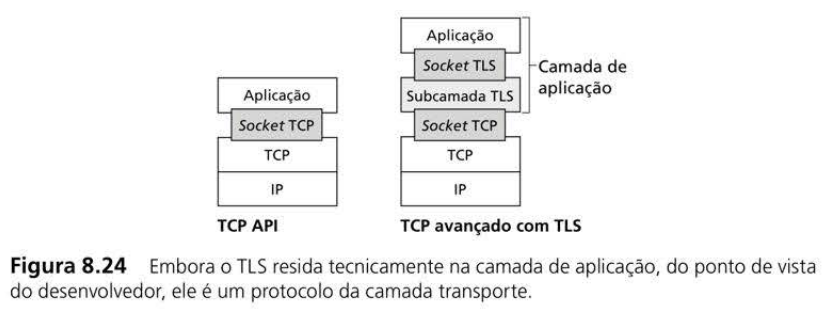
\includegraphics[width=0.9\textwidth]{Figuras/tcp-e-tls.png}


    \end{figure}



\end{frame}

\begin{frame}{Arquitetura do TLS}
    \begin{itemize}
        \item O TLS é projetado para \textbf{usar o TCP} para prover um serviço seguro, confiável (reliable) e fim-a-fim.

        \item O TLS não é um protocolo único, mas sim \textbf{duas camadas} de protocolos.

        \item \textbf{Camada 1: O Protocolo de Registro (Record Protocol)}
              \begin{itemize}
                  \item Fica "em cima" do TCP.
                  \item Fornece os serviços básicos de segurança (criptografia, integridade) para os protocolos da camada superior.
              \end{itemize}

        \item \textbf{Camada 2: Protocolos Superiores (Gerenciamento TLS)}
              \begin{itemize}
                  \item São protocolos \textbf{específicos do TLS}, usados na \textbf{gestão} das trocas TLS.
                  \item São três protocolos que rodam "em cima" do Record Protocol:
                        \begin{itemize}
                            \item Protocolo Handshake (Handshake Protocol)
                            \item Protocolo de Troca de Especificação de Cifra (Change Cipher Spec Protocol)
                            \item Protocolo de Alerta (Alert Protocol)
                        \end{itemize}
              \end{itemize}

        \item \textbf{Camada de Aplicação (Exemplo)}
              \begin{itemize}
                  \item O \textbf{HTTP} (Hypertext Transfer Protocol), usado para interação Web cliente/servidor, pode operar "em cima" do TLS.
              \end{itemize}
    \end{itemize}
\end{frame}

\begin{frame}{A pilha SSL/TLS}


    \begin{figure}
        \centering
        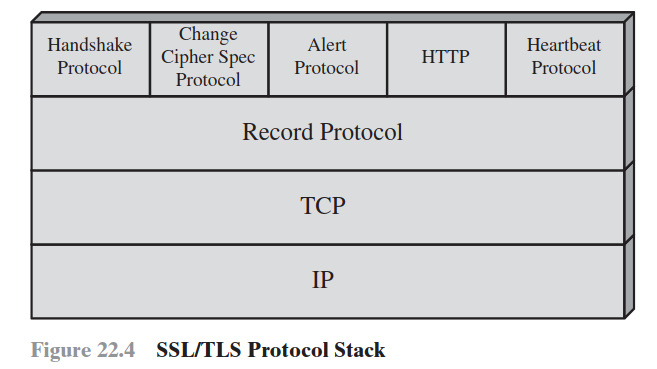
\includegraphics[width=0.7\textwidth]{Figuras/ssl-tls-protocol-stack.png}


    \end{figure}

\end{frame}

\begin{frame}{Conceitos Importantes: Conexão TLS vs. Sessão TLS}
    \begin{itemize}
        \item Existem dois conceitos centrais: Conexão e Sessão.

        \item \textbf{Conexão (Connection)}
              \begin{itemize}
                  \item É um transporte (no sentido OSI) que provê um serviço.
                  \item No TLS, é uma relação \textit{peer-to-peer}.
                  \item As conexões são \textbf{transitórias} (passageiras).
                  \item \textbf{Toda conexão está associada a UMA sessão.}
              \end{itemize}

        \item \textbf{Sessão (Session)}
              \begin{itemize}
                  \item É uma associação entre um cliente e um servidor.
                  \item Criada pelo \textbf{Handshake Protocol}.
                  \item Define um conjunto de \textbf{parâmetros de segurança criptográficos} (chaves, algoritmos, etc.).
                  \item Estes parâmetros podem ser \textbf{compartilhados} entre múltiplas conexões.
                  \item \textbf{Objetivo:} Evitar a negociação (cara) de novos parâmetros de segurança para cada nova conexão.
              \end{itemize}

        \item \textbf{Relacionamento:}
              \begin{itemize}
                  \item Pode haver \textbf{múltiplas conexões seguras} entre um cliente e um servidor.
                  \item Na prática, essas múltiplas conexões compartilham (reutilizam) os parâmetros de uma \textbf{única sessão}.
              \end{itemize}
    \end{itemize}
\end{frame}

\begin{frame}{O protocolo de registro do TLS}


    \begin{figure}
        \centering
        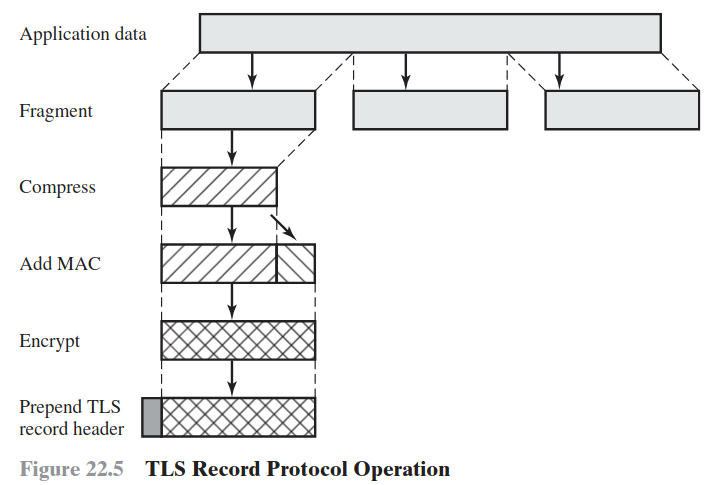
\includegraphics[width=0.7\textwidth]{Figuras/tls-record-protocol.png}


    \end{figure}

\end{frame}

\begin{frame}{Protocolo de Registro TLS (Record Protocol): Serviços}
    \begin{itemize}
        \item O Protocolo de Registro (SSL/TLS Record Protocol) provê dois serviços básicos para as conexões TLS:

        \item \textbf{1. Confidencialidade (Sigilo)}
              \begin{itemize}
                  \item O Protocolo Handshake (visto mais tarde) define uma \textbf{chave secreta compartilhada}.
                  \item Esta chave é usada para \textbf{criptografia simétrica} dos payloads (dados) do TLS.
              \end{itemize}

        \item \textbf{2. Integridade da Mensagem}
              \begin{itemize}
                  \item O Protocolo Handshake também define (outra) \textbf{chave secreta compartilhada}.
                  \item Esta chave é usada para formar um \textbf{MAC (Message Authentication Code)}.
              \end{itemize}

        \item \textbf{Tipos de Conteúdo (Content Types) transportados:}
              \begin{itemize}
                  \item \textit{change\_cipher\_spec} (Protocolo de Gerenciamento TLS)
                  \item \textit{alert} (Protocolo de Gerenciamento TLS)
                  \item \textit{handshake} (Protocolo de Gerenciamento TLS)
                  \item \textit{application\_data} (Dados da Aplicação, ex: HTTP).
              \end{itemize}
        \item \textbf{Obs:} O conteúdo de \textit{application\_data} é \textbf{opaco} para o TLS (ele não sabe o que é HTTP, apenas o protege).
    \end{itemize}
\end{frame}
